\chapter{Результаты исследования}

После предобработки исходного текста из него был сформирован словарь, из которого были отфильтрованы слишком часто или слишком редко встречающиеся слова. Минимальный порог частоты --- 15, максимальный --- 1000. На рисунках \ref{img:1} и  \ref{img:2} представлены гистограммы распределения частот слов в тесте до и после фильтрации. Суммарное число элементов в словаре сократилось с 20333 слов до 2346.

\begin{figure}
	\begin{center}
		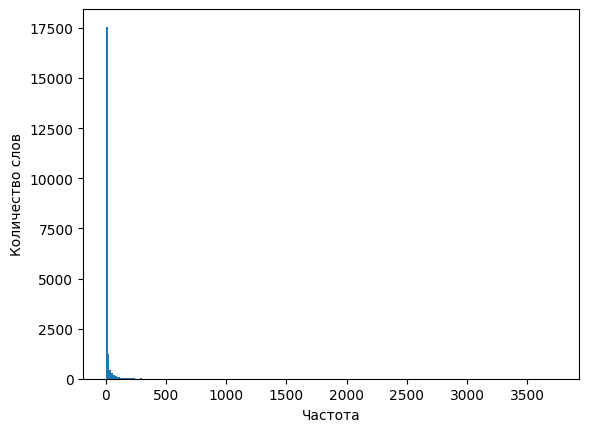
\includegraphics[width=\textwidth]{images/1.png}
	\end{center}
	\caption{Распределение частот слов в тексте до фильтрации}
	\label{img:1}
\end{figure}

\begin{figure}
	\begin{center}
		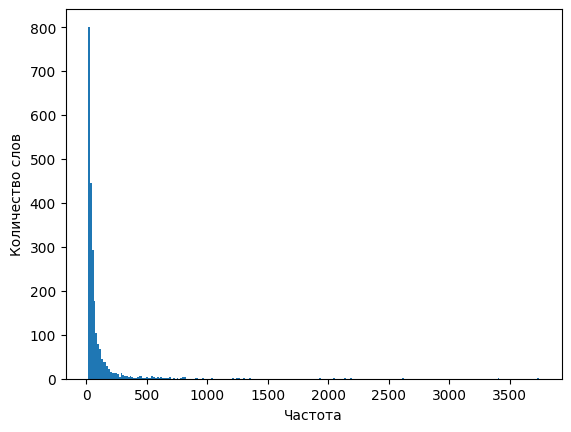
\includegraphics[width=\textwidth]{images/2.png}
	\end{center}
	\caption{Распределение частот слов в тексте после фильтрации}
	\label{img:2}
\end{figure}

Для подбора оптимального количества тем в тексте использовался показатель когерентности тем. Когерентность LDA --- это метрика оценки семантической согласованности тем, измеряющая степень статистической связи между наиболее вероятными словами внутри темы. Высокая когерентность указывает на тесную семантическую связь между топовыми словами темы, что свидетельствует о её содержательной целостности и интерпретируемости. На рисунке \ref{img:3} представлена зависимость когерентности тем от заданного количества тем в тексте. Для дальнейших исследований было взято оптимальное значение --- 18 тем.

\begin{figure}
	\begin{center}
		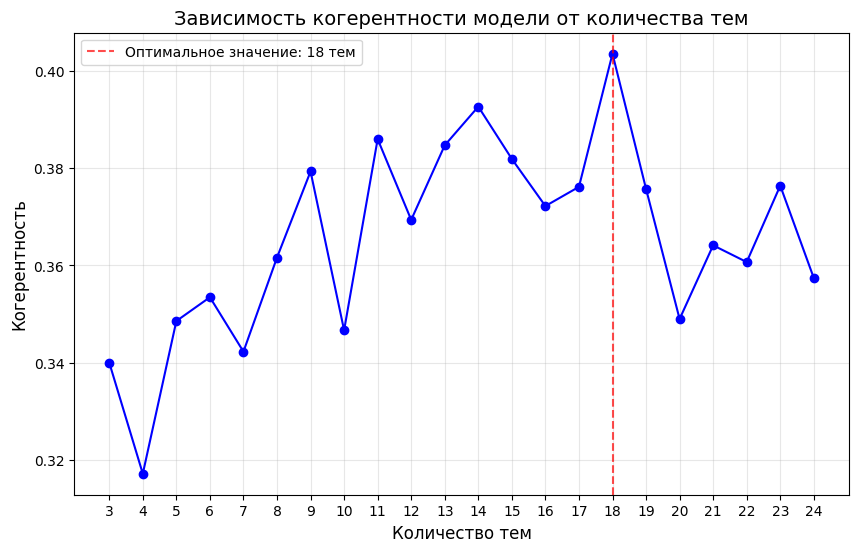
\includegraphics[width=\textwidth]{images/3.png}
	\end{center}
	\caption{Зависимость когерентности тем от заданного количества тем в тексте}
	\label{img:3}
\end{figure}

На рисунке \ref{img:4} представлена визуализация тем в пространстве слов, полученная с помощью алгоритма PCA. Применение данного алгоритма помогло значительно отделить от остальных только темы 4, 5, 10, 15 и 18.

\begin{figure}
	\begin{center}
		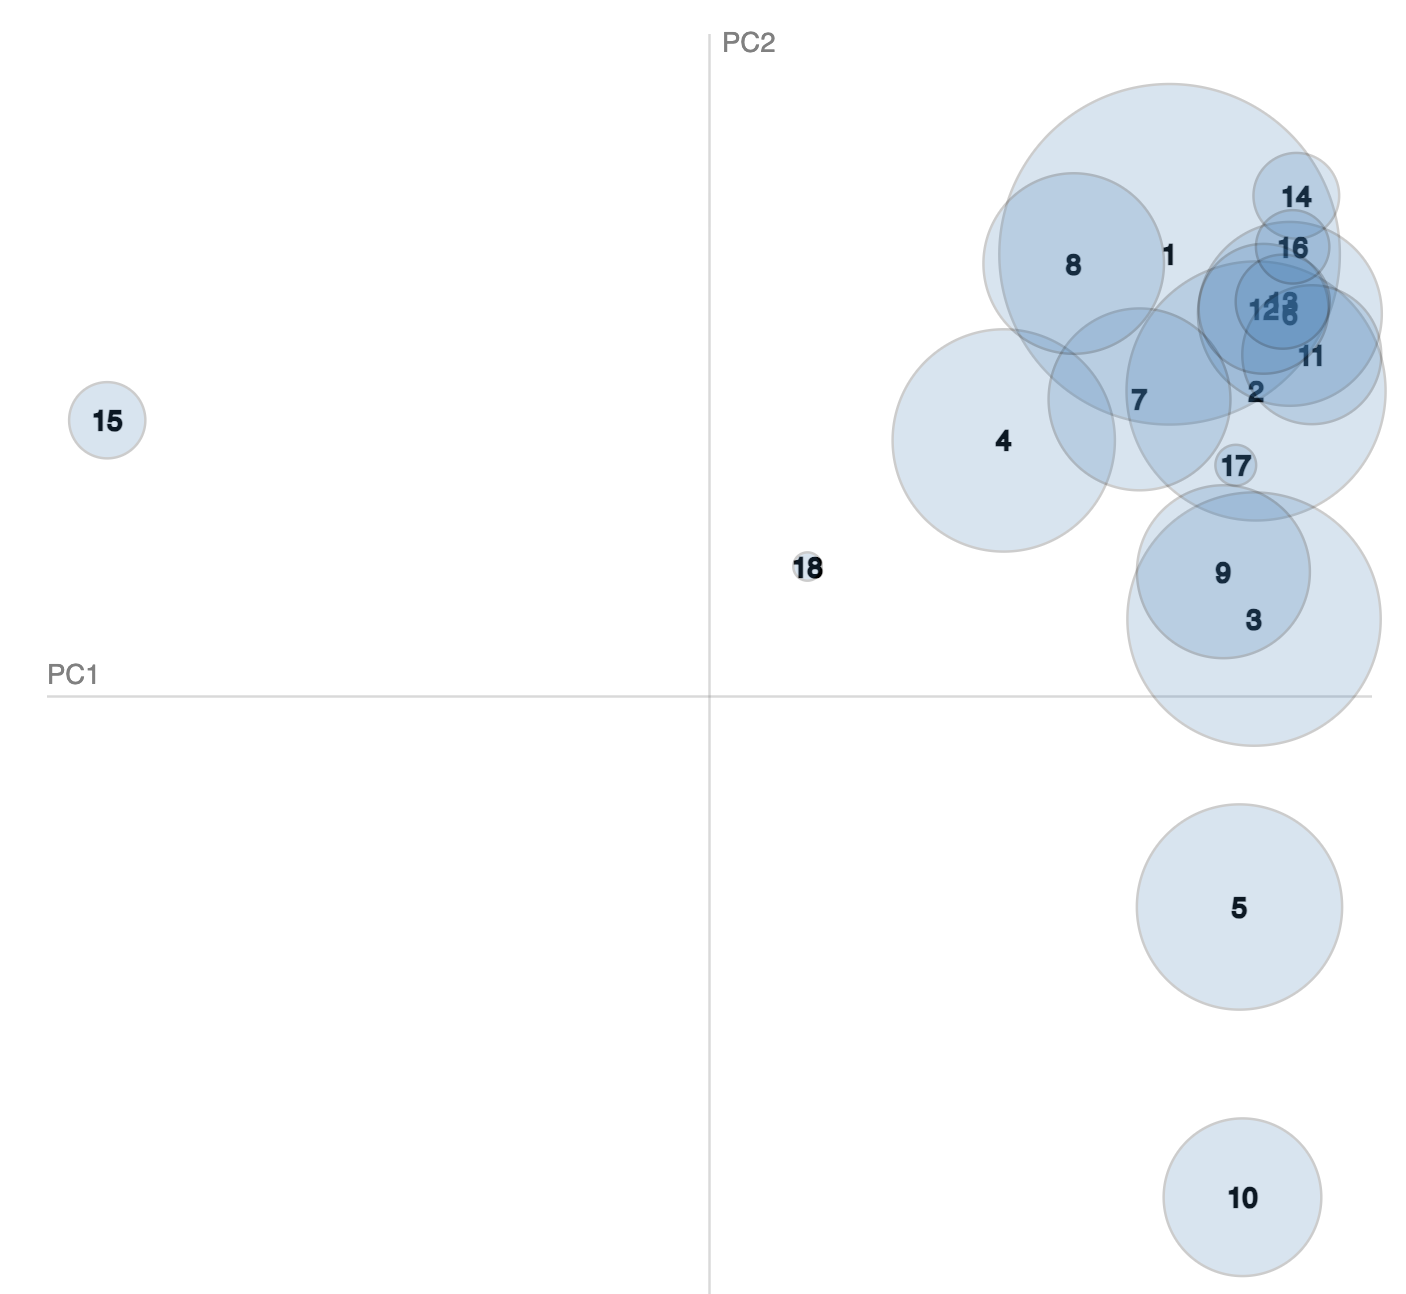
\includegraphics[width=\textwidth]{images/4.png}
	\end{center}
	\caption{Темы в пространстве слов (PCA)}
	\label{img:4}
\end{figure}

На рисунке \ref{img:5} представлена визуализация самых популярных слов в темах, полученная с помощью алгоритма UMAP. Применение данного алгоритма помогло значительно отделить от остальных  все темы текста, кроме 1.

\begin{figure}
	\begin{center}
		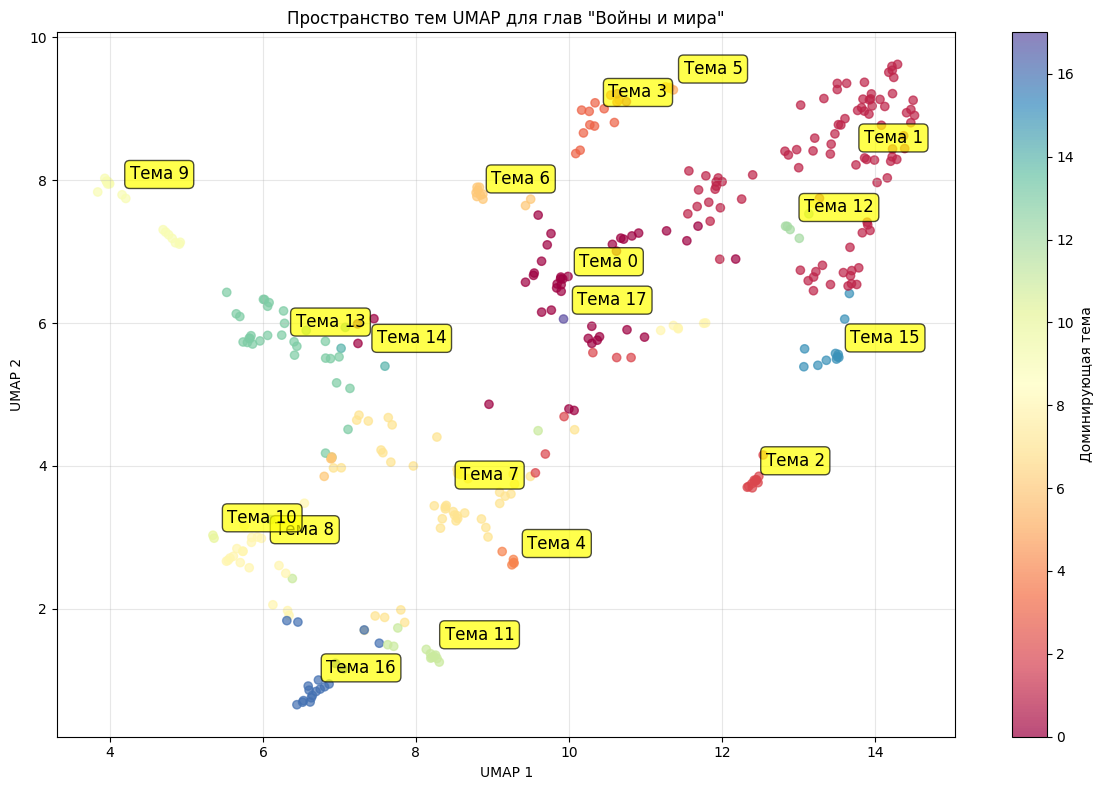
\includegraphics[width=\textwidth]{images/5.png}
	\end{center}
	\caption{Самые популярные слова в каждой теме текста (UMAP)}
	\label{img:5}
\end{figure}

На рисунках \ref{img:6} и  \ref{img:7} представлен анализ сходства тем в тексте.  Среди тем наименее похожей на остальные является тема 10, так как в ней преобладают слова на французском языке.

\begin{figure}
	\begin{center}
		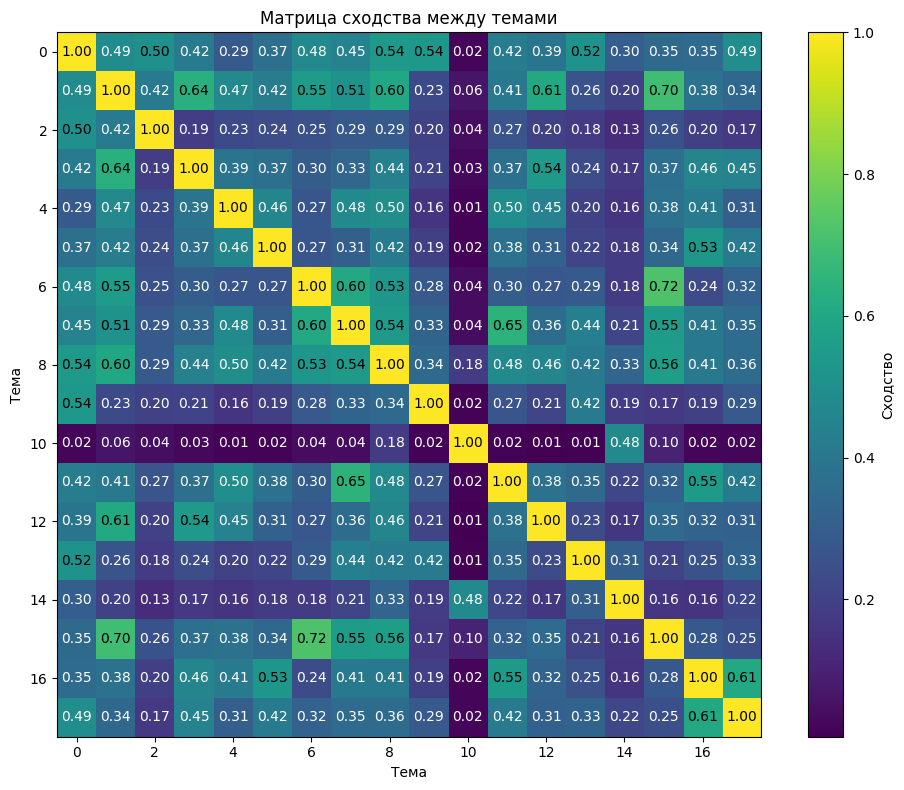
\includegraphics[width=\textwidth]{images/6.png}
	\end{center}
	\caption{Матрица сходства между темами текста}
	\label{img:6}
\end{figure}

\begin{figure}
	\begin{center}
		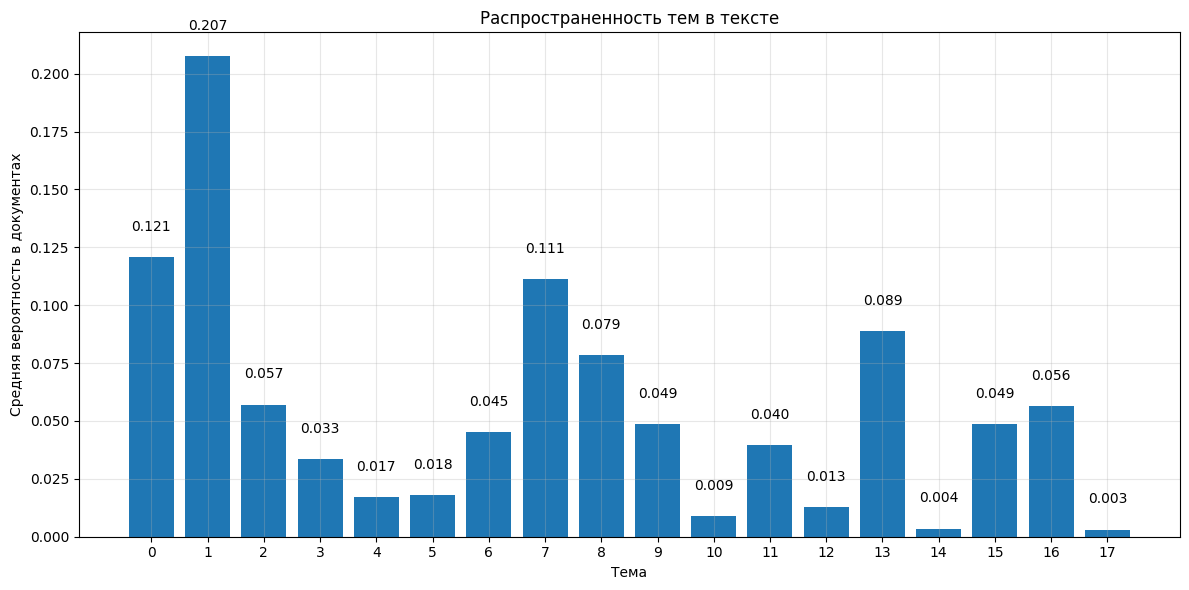
\includegraphics[width=\textwidth]{images/7.png}
	\end{center}
	\caption{Распространённость тем в главах текста}
	\label{img:7}
\end{figure}

\clearpage
